
\documentclass[11pt]{article}

\usepackage[margin=1in]{geometry}
\usepackage{amsmath,amssymb}
\usepackage{siunitx}
\usepackage{graphicx}
\usepackage{booktabs}
\usepackage{enumitem}
\usepackage{hyperref}
\usepackage{tikz}
\usetikzlibrary{arrows.meta,calc,patterns}

\setlist[itemize]{leftmargin=1.2em}
\setlist[enumerate]{leftmargin=1.6em}

\title{\vspace{-1.0em}\textbf{MMAE 450 --- Homework 04: 2D Transient Heat Conduction in a Plate}}
\author{}
\date{\vspace{-1.0em}\textbf{Due: Wednesday, February 4, 2026 (11:59 pm)}}

\begin{document}
\maketitle

%=========================================================
\section*{Problem: Transient Cooling of a Heated Patch in a Rectangular Plate (Dirichlet BCs)}
A thin rectangular plate occupies the domain
\[
0 \le x \le L_x,\qquad 0 \le y \le L_y,
\]
with constant thermal diffusivity $\alpha$. Neglecting through-thickness gradients, the temperature field
$T(x,y,t)$ satisfies the two-dimensional heat equation
\begin{equation}
\frac{\partial T}{\partial t}
=
\alpha\left(\frac{\partial^2 T}{\partial x^2}+\frac{\partial^2 T}{\partial y^2}\right)
\qquad \text{in }\Omega,\; t>0.
\label{eq:heat2d}
\end{equation}

\subsection*{Given data}
Use the following values:
\begin{itemize}
  \item Plate dimensions: $L_x=\SI{1.0}{m}$,\; $L_y=\SI{0.5}{m}$
  \item Thermal diffusivity: $\alpha=\SI{1.0e-4}{m^2/s}$
  \item Uniform grid including boundaries: $N_x=51$, $N_y=26$
\end{itemize}
Thus,
\[
\Delta x=\frac{L_x}{N_x-1},\qquad \Delta y=\frac{L_y}{N_y-1}.
\]

\subsection*{Boundary conditions (Dirichlet on all edges)}
All four edges are held at ambient temperature (take \SI{0}{^\circ C}):
\[
T(0,y,t)=0,\quad T(L_x,y,t)=0,\quad T(x,0,t)=0,\quad T(x,L_y,t)=0.
\]

\subsection*{Initial condition: heated patch}
At $t=0$, the plate is at ambient temperature everywhere \emph{except} for a heated rectangular patch:
\[
T(x,y,0)=
\begin{cases}
100, & 0.45\le x\le 0.55\ \text{and}\ 0.20\le y\le 0.30,\\[0.3em]
0, & \text{otherwise.}
\end{cases}
\]

\subsection*{Geometry and initial condition sketch}
\begin{center}
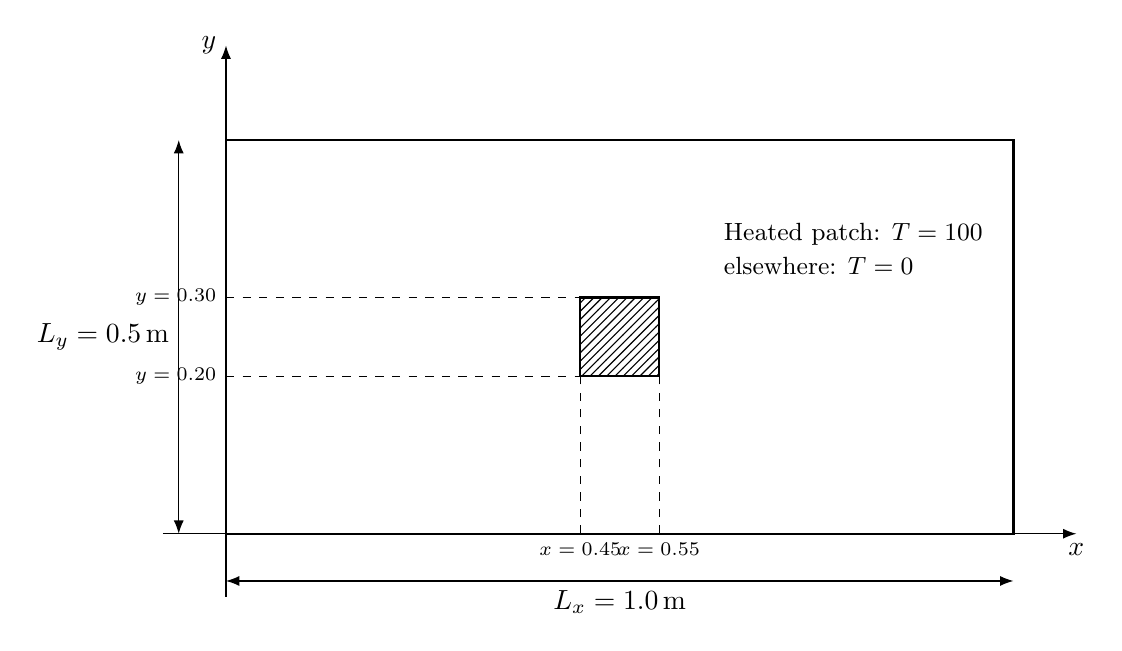
\begin{tikzpicture}[x=10cm,y=10cm,>=Latex]
  % Domain dimensions (scaled to 1 by 0.5)
  \def\Lx{1.0}
  \def\Ly{0.5}

  % Patch bounds
  \def\xa{0.45}
  \def\xb{0.55}
  \def\ya{0.20}
  \def\yb{0.30}

  % Draw plate
  \draw[thick] (0,0) rectangle (\Lx,\Ly);

  % Shade patch
  \fill[pattern=north east lines] (\xa,\ya) rectangle (\xb,\yb);
  \draw[thick] (\xa,\ya) rectangle (\xb,\yb);

  % Axes
  \draw[->] (-0.08,0) -- (1.08,0) node[below] {$x$};
  \draw[->] (0,-0.08) -- (0,0.62) node[left] {$y$};

  % Dimension labels
  \draw[<->] (0,-0.06) -- (\Lx,-0.06) node[midway,below] {$L_x=\SI{1.0}{m}$};
  \draw[<->] (-0.06,0) -- (-0.06,\Ly) node[midway,left] {$L_y=\SI{0.5}{m}$};

  % Patch labels
  \node[anchor=west] at (0.62,0.38) {\small Heated patch: $T=100$};
  \node[anchor=west] at (0.62,0.34) {\small elsewhere: $T=0$};

  % Patch coordinate callouts
  \draw[dashed] (\xa,0) -- (\xa,\ya);
  \draw[dashed] (\xb,0) -- (\xb,\ya);
  \draw[dashed] (0,\ya) -- (\xa,\ya);
  \draw[dashed] (0,\yb) -- (\xa,\yb);

  \node[below] at (\xa,0) {\scriptsize $x=0.45$};
  \node[below] at (\xb,0) {\scriptsize $x=0.55$};
  \node[left] at (0,\ya) {\scriptsize $y=0.20$};
  \node[left] at (0,\yb) {\scriptsize $y=0.30$};

\end{tikzpicture}
\end{center}

%=========================================================
\section*{Numerical method requirement: FTCS}
Use an FTCS discretization of \eqref{eq:heat2d} on the uniform grid:
\begin{equation}
T_{i,j}^{n+1}
=
T_{i,j}^{n}
+\alpha\,\Delta t
\left[
\frac{T_{i+1,j}^{n}-2T_{i,j}^{n}+T_{i-1,j}^{n}}{\Delta x^2}
+
\frac{T_{i,j+1}^{n}-2T_{i,j}^{n}+T_{i,j-1}^{n}}{\Delta y^2}
\right],
\label{eq:ftcs2d}
\end{equation}
for interior nodes $i=1,\dots,N_x-2$ and $j=1,\dots,N_y-2$. Enforce the Dirichlet boundary values at every time step.

\subsection*{Stability requirement}
Your choice of $\Delta t$ must satisfy the 2D FTCS stability condition
\begin{equation}
\alpha\,\Delta t\left(\frac{1}{\Delta x^2}+\frac{1}{\Delta y^2}\right)\le \frac{1}{2}.
\label{eq:stability}
\end{equation}
Choose a ``safe'' $\Delta t$ (e.g.\ some fraction of the maximum stable value) and clearly document it.

%=========================================================
\section*{Deliverables}
Submit \textbf{(i)} a short PDF summary (1--2 pages) and \textbf{(ii)} a Jupyter notebook (\texttt{.ipynb}) that reproduces all results.

\begin{enumerate}
  \item \textbf{Grid and time step.}
  Report $\Delta x$, $\Delta y$, your chosen $\Delta t$, and verify \eqref{eq:stability} numerically.

  \item \textbf{Contour plots.}
  Produce filled contour plots of $T(x,y,t)$ at the following times:
  \[
  t \in \{0,\ 10,\ 50,\ 200\}\ \text{s}.
  \]
  Use consistent contour levels (or a consistent color scale) so the decay is visually clear.

  \item \textbf{Center-point history.}
  Let $(x_c,y_c)=(0.5,0.25)$.
  Plot $T(x_c,y_c,t)$ versus time over the same simulation window.

  \item \textbf{Maximum temperature decay.}
  Compute and plot
  \[
    T_{\max}(t)=\max_{(x,y)\in\Omega} T(x,y,t)
  \]
  versus time.

  \item \textbf{Cooling time metric.}
  Report the first time $t_{10\%}$ at which $T_{\max}(t)$ drops below \SI{10}{^\circ C}.
\end{enumerate}

%=========================================================
\section*{Notes and good practice}
\begin{itemize}
  \item Use clear variable names and consistent indexing ($i$ for $x$, $j$ for $y$).
  \item Boundary nodes are prescribed values (not unknowns). Enforce them directly.
  \item Include at least one brief code cell that prints a quick stability check value:
  \[
    \eta=\alpha\,\Delta t\left(\frac{1}{\Delta x^2}+\frac{1}{\Delta y^2}\right)
    \quad \text{and confirm}\quad \eta\le \frac{1}{2}.
  \]
\end{itemize}

%=========================================================
\section*{Optional extension (extra credit)}
Implement a fully implicit method (Backward Euler or Crank--Nicolson) in 2D and solve the linear system at each time step using Gauss--Seidel (or SOR). Compare:
\begin{itemize}
  \item allowable time steps,
  \item runtime,
  \item accuracy of the temperature histories.
\end{itemize}

\end{document}
